% Copyright 2004 by Till Tantau <tantau@users.sourceforge.net>.
%
% In principle, this file can be redistributed and/or modified under
% the terms of the GNU Public License, version 2.
%
% However, this file is supposed to be a template to be modified
% for your own needs. For this reason, if you use this file as a
% template and not specifically distribute it as part of a another
% package/program, I grant the extra permission to freely copy and
% modify this file as you see fit and even to delete this copyright
% notice. 

% --------------------------------------------
% Template por Patricio López Juri (pelopez2@uc.cl)

% Slides con pausas
\documentclass[spanish]{beamer}

% Slides sin pausas
% \documentclass[spanish,handout]{beamer}


%% -----------------------------------------------------
%% Python & código -------------------------------------
%% -----------------------------------------------------

% Source: https://github.com/bamos/beamer-snippets

\usepackage[T1]{fontenc}
\usepackage{parskip,graphics,tikz,multimedia,hyperref,ulem,multicol}
\usetikzlibrary{arrows,positioning,shapes,decorations.pathmorphing,snakes}
\setlength{\itemsep}{0pt}\setlength{\parskip}{0pt}\setlength{\parsep}{0pt}
\graphicspath{{./images/}}

\usepackage{listings,textcomp,color}
\lstset{language=Python,upquote=true,
  basicstyle=\ttfamily\footnotesize,numbers=left,
  numberstyle=\tiny,stepnumber=1,numbersep=5pt,
  backgroundcolor=\color{white},frame=single,tabsize=2,
  showspaces=false,showstringspaces=false,showtabs=false,
  breaklines=true,breakatwhitespace=true,escapeinside=||,
  keywordstyle=\color{blue!70},stringstyle=\color{green!70!black!70},
  commentstyle=\color{black!80}\it
}

\usebackgroundtemplate{
  \tikz[overlay,remember picture]
  \node[yshift=10mm,anchor=south east,inner sep=0pt]
    at (current page.south east) {
    % Add small logo here if desired.
    % \includegraphics[width=0.5in]{Images/python-logo.png}
  };
}

\tikzset{
  yn/.style={draw,thick,rounded corners,fill=yellow!20,inner sep=.3cm},
  bn/.style={draw,thick,rounded corners,fill=blue!05,inner sep=.3cm},
  on/.style={draw,thick,rounded corners,fill=orange!20,inner sep=.3cm},
  rn/.style={draw,thick,rounded corners,fill=red!20,inner sep=.3cm},
  greenn/.style={draw,thick,rounded corners,fill=green!20,inner sep=.3cm},
  grayn/.style={draw,thick,rounded corners,fill=gray!20,inner sep=.3cm},
  to/.style={
    ->,>=stealth',shorten >=1pt,semithick,font=\sffamily\footnotesize
  },
  from/.style={
    <-,>=stealth',shorten >=1pt,semithick,font=\sffamily\footnotesize
  },
  tofrom/.style={
    <->,>=stealth',shorten >=1pt,semithick,font=\sffamily\footnotesize
  },
  every node/.style={align=center},
  squig/.style={->,line join=round,decorate, decoration={zigzag,
    segment length=8,amplitude=2,post=lineto,post length=2pt}}
}

\newcommand{\uncheckedBox}{\ensuremath{\square}}
\newcommand{\checkedBox}{\ensuremath{\text{\rlap{\checkmark}}\square}}

\beamertemplatenavigationsymbolsempty

\expandafter\def\expandafter\insertshorttitle\expandafter{%
  \insertshorttitle\hfill%
  \insertframenumber\,/\,\inserttotalframenumber}

\usepackage{enumitem}
\setlist[1]{itemsep=5pt}
\setitemize{label=\usebeamerfont*{itemize item}%
  \usebeamercolor[fg]{itemize item}
  \usebeamertemplate{itemize item}}
  
  
%% -----------------------------------------------------
%% Lenguaje --------------------------------------------
%% -----------------------------------------------------

% \usepackage[T1]{fontenc} Está mas arriba.
\usepackage{selinput}
\SelectInputMappings{%
  aacute={á},
  ntilde={ñ},
  Euro={€}
}
\usepackage[spanish]{babel}


%% -----------------------------------------------------
%% Tema ------------------------------------------------
%% -----------------------------------------------------

% Colores principales
\usetheme{CambridgeUS}

% Para las URL
\definecolor{links}{HTML}{2A1B81}
\hypersetup{colorlinks,linkcolor=,urlcolor=links}


%% -----------------------------------------------------
%% Main ------------------------------------------------
%% -----------------------------------------------------

% Título, debe ir obligatoriamente
\title{Ayudantía 09}

% Subtítulo opcional
\subtitle{Threading}

% Ayudantes
\author{Felipe Garrido \and Vicente Domínguez}

% Universidad
\institute[UC]
{
  Departmento de Ciencia de la Computación\\
  Pontificia Universidad Católica de Chile
}

% Dimensión tiempo espacio a mostrar.
\date{IIC2233, 2015-1}

% Metadada
\subject{Ayudantía de Programación Avanzada}


% If you have a file called "university-logo-filename.xxx", where xxx
% is a graphic format that can be processed by latex or pdflatex,
% resp., then you can add a logo as follows:

% \pgfdeclareimage[height=0.5cm]{university-logo}{university-logo-filename}
% \logo{\pgfuseimage{university-logo}}

% Delete this, if you do not want the table of contents to pop up at
% the beginning of each subsection:
% \AtBeginSubsection[]
% {
%   \begin{frame}<beamer>{Outline}
%     \tableofcontents[currentsection,currentsubsection]
%   \end{frame}
% }


%% -----------------------------------------------------
%% Incio del documento ---------------------------------
%% -----------------------------------------------------

\begin{document}

% Agregamos la página de inicio (la del título)
\begin{frame}
  \titlepage
\end{frame}

% Tabla de contenidos, tiene hipervínculos.
% Los índices son tomados del nombre que se le asigne a las \section.
% Los sub-índices provienen de las \subsections
\begin{frame}{Tabla de contenidos}
  \tableofcontents
  % You might wish to add the option [pausesections]
\end{frame}


%% **********************
%% Sección **************
%% **********************
\section{¿Qué son los threads?}

\subsection{Definición y usos}


\begin{frame}{¿Qué son los threads?}
  \begin{center}
    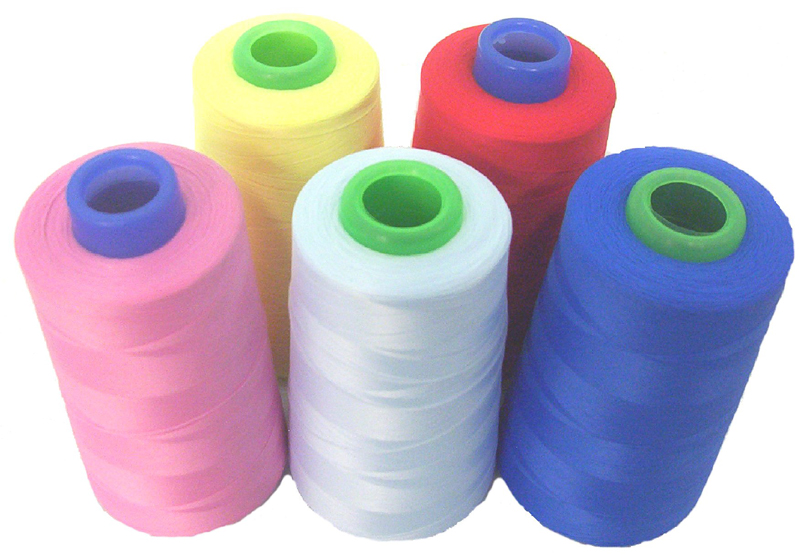
\includegraphics[height=6cm]{Images/hilos.jpg}
    \\
    ¿Hilos?.
  \end{center}
\end{frame}

\begin{frame}{¿Qué son los threads?}
  \begin{center}
    
\includegraphics[height=6cm]{Images/pelicula.jpg}
    \\
    ¿Una película?.
  \end{center}
\end{frame}

\begin{frame}{¿Qué son los threads?}
  \begin{center}
    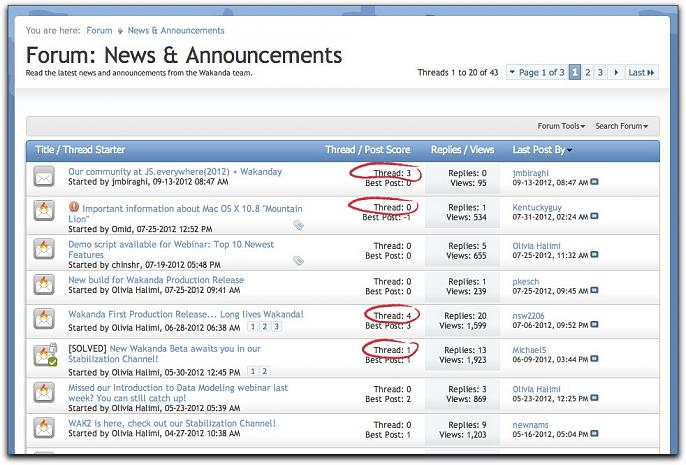
\includegraphics[height=6cm]{Images/foros.jpg}
    \\
    ¿Conversaciones? Esto se asemeja un poco más.
  \end{center}
\end{frame}

\begin{frame}{¿Qué son los threads?}
  \begin{center}
    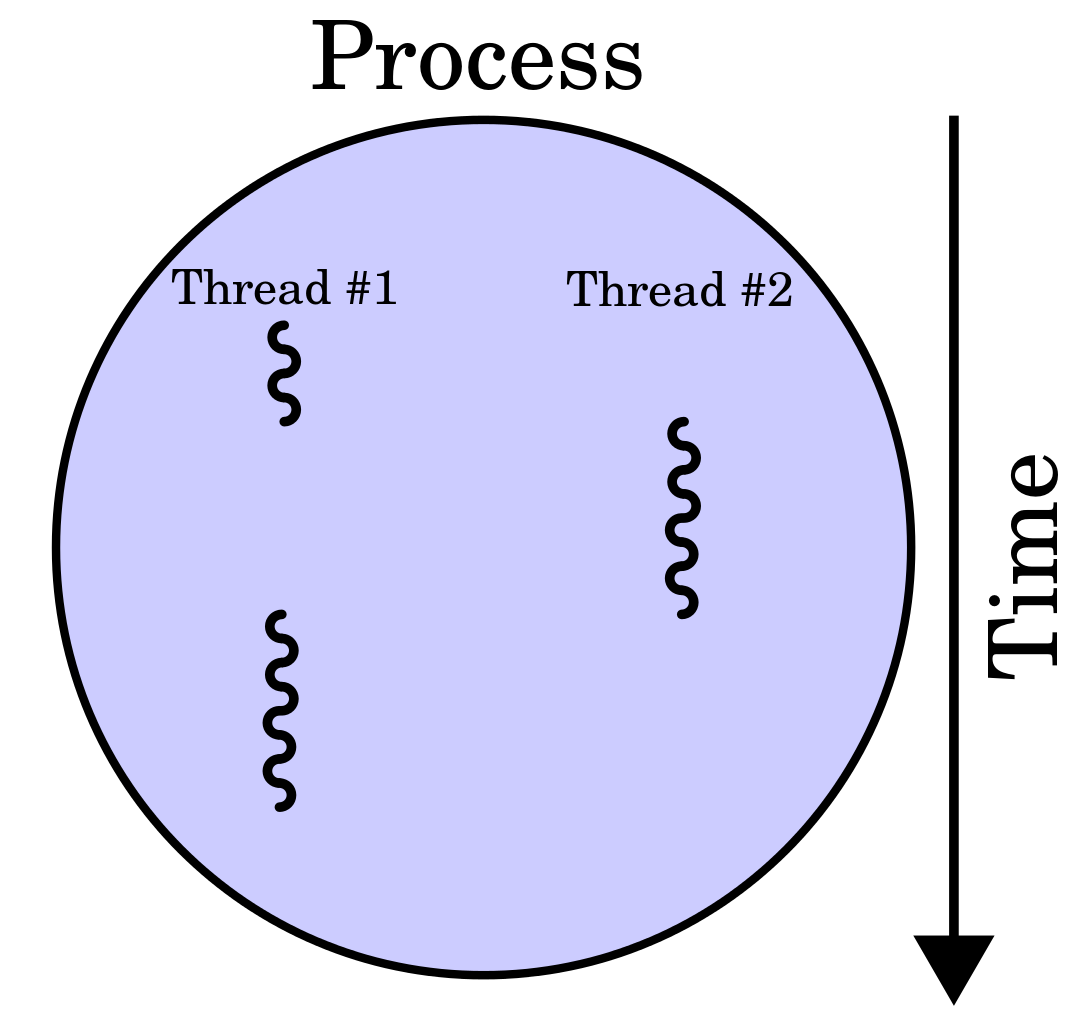
\includegraphics[height=6cm]{Images/thread.png}
    \\
    En computación, esto es lo que entenderemos como threads.
  \end{center}
\end{frame}

\begin{frame}{¿Qué son los threads?}{Definición y usos}
  \begin{itemize}
  \item
    En ciencia de la computación entenderemos un \alert{thread} como la unidad básica de procesamiento que puede ser ejecutada o planificada por un sistema operativo.
  \item
    Los threads son parte de un \textit{proceso}. En palabras simples este puede entenderse como un programa en ejecución, o formalmente como \textit{Una unidad de actividad que se caracteriza por la ejecución de una secuencia de instrucciones, un estado actual, y un conjunto de recursos del sistema asociados }(Stallings 5º edición pag. 109).
  \end{itemize}
\end{frame}

\begin{frame}{¿Qué son los threads?}{Definición y usos}
  \begin{itemize}
  \item
    En general cuando se ejecuta un programa en un computador este no se corre de forma lineal, más bien hay una serie de procesos funcionando a la vez de forma \textit{"pseudoparalela"}.
  \item
    Los \alert{threads} nos permiten generar este \textit{pseudoparalelismo} en nuestro programa y nos dan la capacidad de ejecutar multiples tareas de forma simultanea.
  \item
    En \alert{Python}, y en la mayoría de los lenguajes de programación, la forma de usar los \alert{threads} es creando a una variable del tipo \alert{thread}, a esta se le asigna una función o método a ejecutar y luego se inicializa este. De esta forma el código principal sigue ejecutandose mientras el \alert{thread} también sigue de forma \textit{pseudoparalela}.
  \end{itemize}
\end{frame}




%% **********************
%% Sección **************
%% **********************
\section{Threads en Python}

%% Sub-sección 
%% **********************
\subsection{Sintaxis}

\begin{frame}[fragile]{Threads en Python}{Sintaxis}
  Código ejemplo
  \begin{lstlisting}[language=Python]
import threading

def sumainfinita(a,b):
    while True:
        c = a + b
        print(c)

t_1 = threading.Thread(target=sumainfinita, args=(a,b))
t_1.daemon = True
t_1.start()

  \end{lstlisting}
\end{frame}


\section{Multithreading}

\subsection{Mecanismos de sincronización}

\begin{frame}{Multithreading}
  \begin{itemize}
  \item
    El uso de \alert{multithreading} puede resultar muy útil para acelerar la ejecución de un programa o para lograr de que cumpla lo requerido.
  \item
    Aunque tenga muchos beneficios esta práctica, también acarrea problemas.
  \item
    Los principales son la coordinación de los \alert{threads} (lograr de que uno ejecute en ciertos momentos del otro) y las colisiones entre ellos (cuando más de uno intenta acceder a una sección de código simultaneamente).
  \end{itemize}
\end{frame}

\begin{frame}{Multithreading}
  \begin{center}
    
\includegraphics[height=6cm]{Images/puppies.png}
    \\
    En la práctica...
  \end{center}
\end{frame}

\begin{frame}{Multithreading}
  \begin{center}
    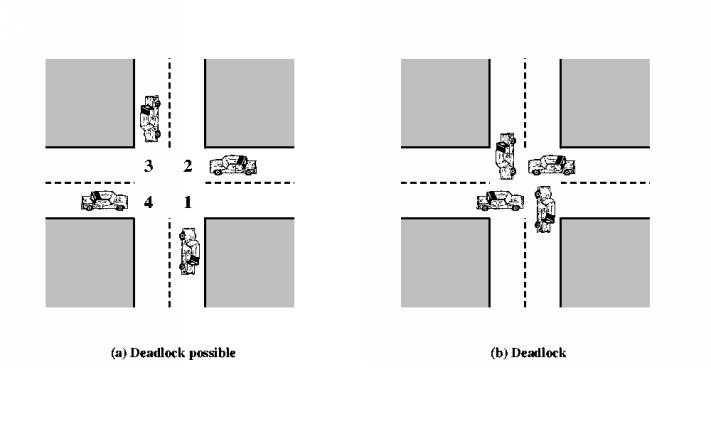
\includegraphics[height=6cm]{Images/deadlock1.jpg}
    \\
    Deadlock en la teoría.
  \end{center}
\end{frame}

\begin{frame}{Multithreading}
  \begin{center}
    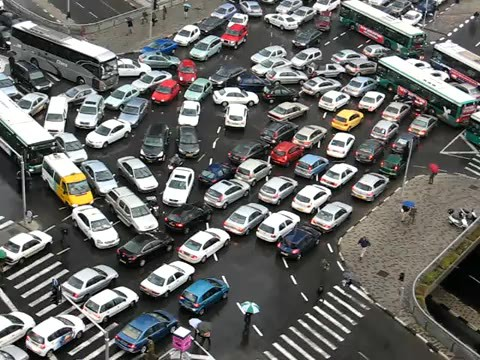
\includegraphics[height=6cm]{Images/deadlock2.jpg}
    \\
    Deadlock en la práctica.
  \end{center}
\end{frame}

\begin{frame}{Multithreading}
  \begin{center}
    
\includegraphics[height=6cm]{Images/theysaid.jpg}
    \pause
    \\
    ¿Qué podemos hacer?
  \end{center}
\end{frame}

\begin{frame}{Multithreading}{Mecanismos de sincronización}
  \begin{itemize}
  \item
    Como estos son problemas recurrentes, existes mecanismos de sincronización de \alert{threads}.
  \item
    Estos mecanismos nos permiten tener un mayor control sobre los \alert{threads} y así poder evitar las colisiones u otros problemas similares.
  \item
    Uno muy recurrente en los lenguajes de programación es el \alert{lock}. Este consiste en encapsular una sección de código (generalmente una sección que ocasione problemas entre los \alert{threads}) y solo permitir el acceso de un \alert{threads} a la vez a esa parte del programa.
  \end{itemize}
\end{frame}

\begin{frame}[fragile]{Multithreading}{Sintaxis}

Código ejemplo:
  \begin{lstlisting}[language=Python]
import threading

lock = threading.Lock()

def funcioninteresante():
    ...
    lock.acquire()
    ...
    # zona de conflicto
    ...
    lock.release()
    ...
  \end{lstlisting}
\end{frame}

\begin{frame}[fragile]{Multithreading}{Sintaxis}

Código ejemplo:
  \begin{lstlisting}[language=Python]
import threading

lock = threading.Lock()

def funcioninteresante():
    ...
    with lock:
        # zona de conflicto
    ...
  \end{lstlisting}
\end{frame}

\end{document}
